%%This is a very basic article template.
%%There is just one section and two subsections.
\documentclass{article}
\usepackage{graphicx}
\usepackage{amsmath}
\begin{document}
\title{Photocurrent Action spectra of Photovotaic Devices}
\maketitle
\section{Internal Optical electric field and energy dissipation due to an incident plane wave
}

\subsection{Transfer Matrix Method:~\cite{pettersson1999modeling}}

Stratified structures can be described by $2\times2$ matrix 
due to the fact that the equation governing the propagation 
of the electric field are linear and that the tangential component 
of the electric field is continuous.Consider a plane wave incident from left at a general multilayer 
structure having m layers between a semi-infinite transparent ambient 
and a semi-infinite substrate as schematically described in Figure
\ref{fig:layers}.
\begin{figure}[h!]
  \centering
    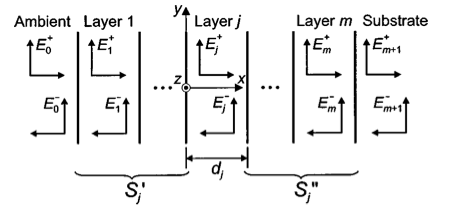
\includegraphics[width=0.7\textwidth]{layers}
  \caption{A general multilayer structure having m layers between a semi 
  infinite transparent ambient and a semi-infinite substrate. 
 Each layer j(j=1,2,…,m) has a thickness $d_{j}$ and its optical properties are
 described by its complex index of refraction. The optical electric field at any
 point in lyaer j is represented by two components: one propagating in the
 positive and one in the negative x direction, $\mathbf{E_{j}^{+}}$ and
 $\mathbf{E_{j}^{-}}$, respectively} \label{fig:layers} 
\end{figure}
\subsubsection{Theoretical Background}
The electric field in layer j can be expressed in terms of the matrix elements
of the partial system transfer matrices as

\begin{equation}
{{E}_{j}}(x)=\frac{S_{j11}^{''}\cdot {{e}^{-i{{\xi
}_{j}}({{d}_{j}}-x)}}+S_{j21}^{''}\cdot {{e}^{i{{\xi }_{j}}({{d}_{j}}-x)}}}{S_{j11}^{'}S_{j11}^{''}\cdot {{e}^{-i{{\xi }_{j}}{{d}_{j}}}}+S_{j12}^{'}S_{j21}^{''}\cdot {{e}^{i{{\xi }_{j}}{{d}_{j}}}}}E_{0}^{+}
\label{mainequation} 
\end{equation}
In Equation \ref{mainequation}:

$d_j$ is the thickness of the jth layer as shown in Figure \ref{fig:layers}.
\begin{equation}
{{\xi }_{j}}=\frac{2\pi }{\lambda }{{q}_{j}}
\end{equation}
\begin{equation}
S_{j}^{'}=\left[ \begin{matrix}
   S_{j11}^{'} & S_{j12}^{'}\\
   S_{j21}^{'} & S_{j22}^{'}  
\end{matrix} \right]=\left( \prod\limits_{v=1}^{j-1}{{{I}_{(v-1)v}}{{L}_{v}}} \right)\cdot {{I}_{(j-1)j}}
\label{Sp} 
\end{equation}
\begin{equation}
S_{j}^{''}=\left[ \begin{matrix}
   S_{j11}^{''} & S_{j12}^{''}\\
   S_{j21}^{''} & S_{j22}^{''}\\
\end{matrix} \right]=\left( \prod\limits_{v=j+1}^{m}{{{I}_{(v-1)v}}{{L}_{v}}} \right)\cdot {{I}_{m(m+1)}}
\label{Spp} 
\end{equation}
\begin{equation}
{{I}_{jk}}=\frac{1}{{{t}_{jk}}}\left[ \begin{matrix}
   1 & {{r}_{jk}}  \\
   {{r}_{jk}} & 1  \\
\end{matrix} \right]
\end{equation}
\begin{equation}
{{L}_{j}}=\left[ \begin{matrix}
   {{e}^{-i{{\xi }_{j}}{{d}_{j}}}} & 0  \\
   0 & {{e}^{i{{\xi }_{j}}{{d}_{j}}}}  \\
\end{matrix} \right]
\end{equation}
For light with the electric field perpendicular to the plane of
incidence(s-polarized or TE waves), the Fresnel complex reflection and
transmission coefficients are defined by
\begin{subequations}
\begin{equation}
{{r}_{jk}}=\frac{{{q}_{j}}-{{q}_{k}}}{{{q}_{j}}+{{q}_{k}}}
\end{equation}
\begin{equation}
{{t}_{jk}}=\frac{2{{q}_{j}}}{{{q}_{j}}+{{q}_{k}}}
\end{equation}
\end{subequations}



\subsection{Another subtitle}
More plain text.

\bibliography{mybib}{}
\bibliographystyle{plain}
\end{document}
